\section{Results}

In this section, we will present the combined results of our work. We will start by discussing the results of the PyTorch fuzzing campaign, then we will take a look at the experimental results for the proposed hybrid fuzzer improvements, in particular, the scheduling strategy. Finally, we will discuss the results of the improved annotation mechanism.

\subsection{PyTorch Findings} \label{results:pytorch-findings}

The first and foremost achievement of this thesis is the discovery of bugs and vulnerabilities in the PyTorch framework.

During the PyTorch fuzzing campaign, we were able to find a total of 17 unique bugs, all of which were confirmed and fixed. The bugs were found in various PyTorch modules, including the \textit{unpickler}, the \textit{irparser}, and the distributed communication library. The bugs were reported to the PyTorch team and were fixed in the following pull requests:

\begin{itemize}
    \item \href{https://github.com/pytorch/pytorch/pull/94300}{\#94300: Add size check before calling stack\_.at(dict\_pos) in unpickler.cpp}
    \item \href{https://github.com/pytorch/pytorch/pull/94298}{\#94298: Add stack emptiness checks inside interpreter.cpp}
    \item \href{https://github.com/pytorch/pytorch/pull/94297}{\#94297: Add size check before calling .back() in rpc/script\_call.cpp}
    \item \href{https://github.com/pytorch/pytorch/pull/94295}{\#94295: Add exception handlers for stoll in schema\_type\_parser.cpp}
    \item \href{https://github.com/pytorch/pytorch/pull/91401}{\#91401: Add out-of-bounds checks inside irparser.cpp and unpickler.cpp}
\end{itemize}

In the following subsections, we will take a closer look at some bugs.

\subsubsection{\#94297: Out-of-bounds access in rpc/script\_call.cpp}

One of the most significant findings from our fuzzing campaign was bug \#94297, which was discovered in the \textit{rpc} module of PyTorch. This bug resulted from an out-of-bounds access in the \textit{ScriptCall::fromIValues} function, where the function attempted to access the last element of the \textit{ivalues} vector without first checking if the vector was empty. The result was a segmentation fault. To fix the issue, we added a size check to ensure that the vector's size was greater than one. The patch for this bug can be seen in Listing \ref{listing:pytorch-bug-94297-patch}.

\begin{listing}[h!]
    \centering
    \begin{minipage}{\linewidth}
        \begin{minted}[linenos=true, tabsize=2, breaklines=true]{diff}
std::unique_ptr<ScriptCall> ScriptCall::fromIValues(
    std::vector<at::IValue>& ivalues) {
+  TORCH_INTERNAL_ASSERT(
+      ivalues.size() > 1,
+      "At least 2 IValues are required to build a ScriptCall.");
    \end{minted}
    \end{minipage}
    \caption{Patch for bug \#94297}
    \label{listing:pytorch-bug-94297-patch}
\end{listing}

This bug is an interesting example to analyze, as it has the potential to cause a denial of service attack in the best-case scenario, and in the worst-case scenario, it could enable an attacker to execute code remotely.

\subsubsection{\#91401: Out-of-bounds access in irparser.cpp and unpickler.cpp}

Another interesting discovery that we made was fixed in pull-request \#91401. We found multiple out-of-bounds accesses in the \textit{irparser} and \textit{unpickler} modules of PyTorch. Of particular interest were the bugs in the \textit{unpickler} module, as they could be triggered by a malicious pickle payload, either by loading a malicious \textit{.pt} model or by parsing a malicious RPC payload sent over the network. Part of the patch for this bug can be seen in Listing \ref{listing:pytorch-bug-91401-patch}.

\begin{listing}
    \centering
    \begin{minipage}{0.9\linewidth}
        \begin{minted}[linenos=true, tabsize=2, breaklines=true, fontsize=\small]{diff}
    case PickleOpCode::NEWOBJ: {
+     TORCH_CHECK(!stack_.empty(), "Parsing error: stack_ is empty");
      // pop empty tuple, the actual action is stored in the globals_stack_
      stack_.pop_back();
    } break;
@@ -466,6 +474,7 @@ PickleOpCode Unpickler::readInstruction() {
      globals_.at(idx)();
    } break;
    case PickleOpCode::BINPERSID: {
+     TORCH_CHECK(!stack_.empty(), "Parsing error: stack_ is empty");
      auto tuple = pop(stack_).toTuple();
      const auto& args = tuple->elements();
      AT_ASSERT(
    \end{minted}
    \end{minipage}
    \caption{Patch for bug unpickler bugs in \#91401}
    \label{listing:pytorch-bug-91401-patch}
\end{listing}

\subsubsection{Positive Hack Days Talk}

Apart from conducting a thorough security analysis of PyTorch and discovering many bugs, we have also decided to share our findings and methodology with the security community. We submitted a talk proposal titled "Spotting Bugs in PyTorch with Continuous Fuzzing" to the Positive Hack Days (PHD) 2023 conference organizing committee, and it was accepted. Our talk is scheduled to be presented at the conference in Moscow, Russia on May 19-20, 2023. By sharing our insights with the broader community, we hope to raise awareness about the importance of continuous fuzzing and inspire others to adopt similar approaches in their security analysis efforts.

In conclusion to this section, we believe that our fuzzing campaign was a success. We were able to find multiple bugs in PyTorch, all of which were confirmed and fixed. We also are going to share our findings with the broader security community by presenting a talk at the Positive Hack Days conference.

\subsection{Experimental Results for the Scheduling Strategy} \label{results:symbolic-pointers-modeling-scheduling}

The next important contribution of this thesis is the development of a scheduling strategy for the \textit{sydr-fuzz}, and the experimental evaluation of its performance.

To find that the optimal value for the scheduling strategy's parameter N is 25, we have conducted a series of experiments on the \textit{Fuzzbench} platform. We have tested 3 different configurations:

\begin{itemize}
    \item \textbf{symptr-15}: Sydr with enabled memory modeling, $N=15$ vs Sydr with disabled memory modeling
    \item \textbf{symptr-25}: Sydr with enabled memory modeling, $N=25$ vs Sydr with disabled memory modeling
    \item \textbf{symptr-25-vs-35}: Sydr with enabled memory modeling, $N=25$ vs Sydr with enabled memory modeling, $N=35$
\end{itemize}

We have run each configuration for 23 hours with 10 trials per fuzzer. After that the results were collected and different metrics were calculated. In particular, the average score with the average rank, and the median relative code coverage for each benchmark.

\subsubsection{symptr-15}

The results for the first configuration are shown in Figures \ref{fig:fuzzbench-symptr-15-1-coverage} and \ref{fig:fuzzbench-symptr-15-1-score-rank}. Coverage growth graphs can be found in Appendix \ref{fig:fuzzbench:symptr-15-1}.

\begin{figure}[h]
    \centering
    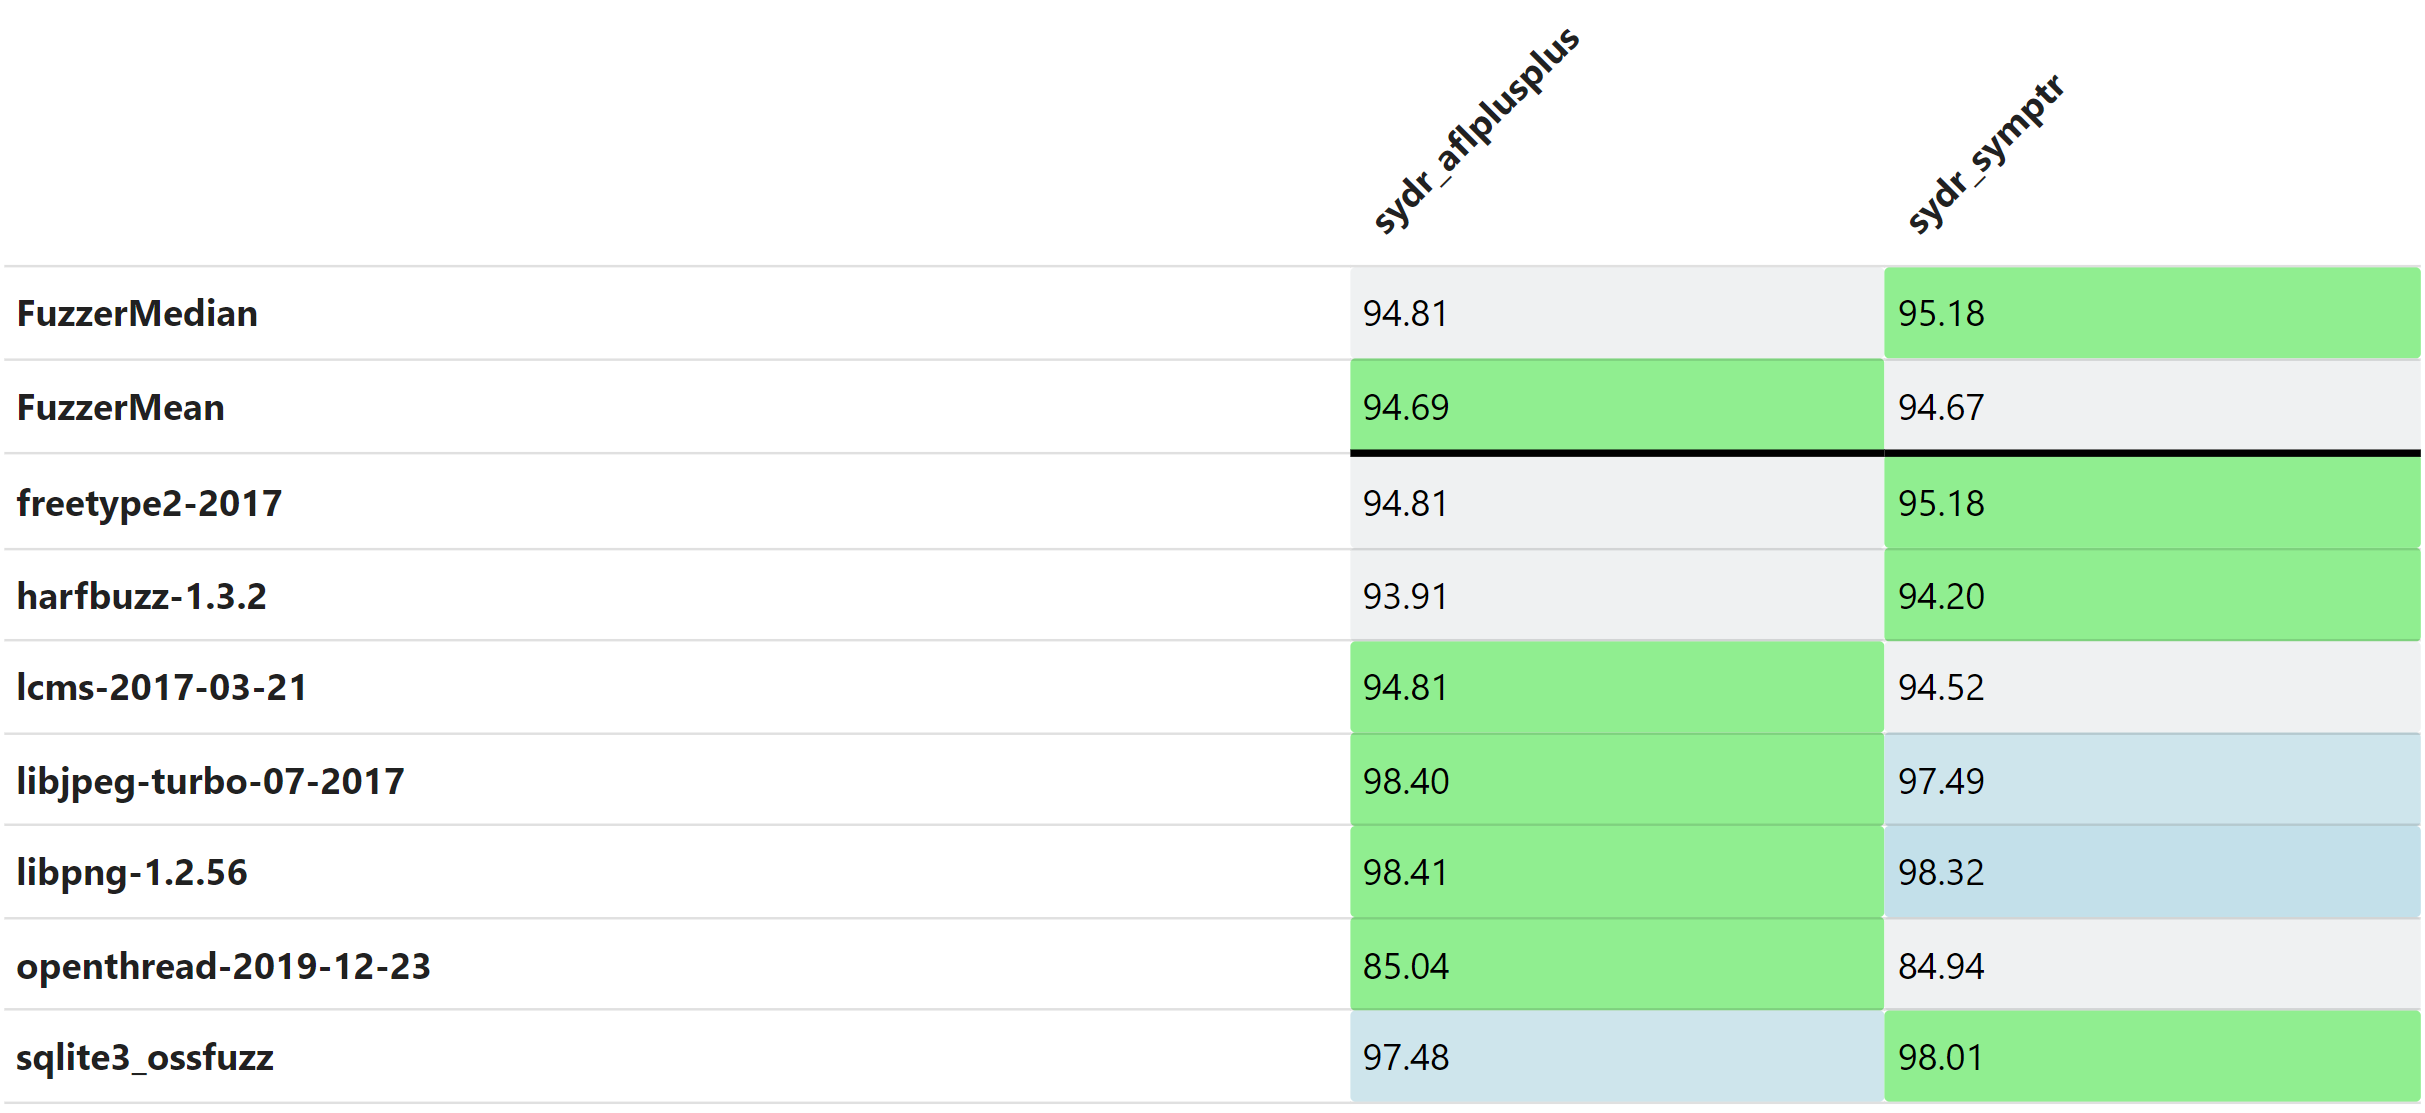
\includegraphics[width=0.9\textwidth]{assets/fuzzbench/symptr-15-1/median-relative-code-coverage-on-each-benchmark.png}
    \caption{Median relative code coverage on each benchmark ($N=15$)}
    \label{fig:fuzzbench-symptr-15-1-coverage}
\end{figure}

\begin{figure}[h]
    \centering
    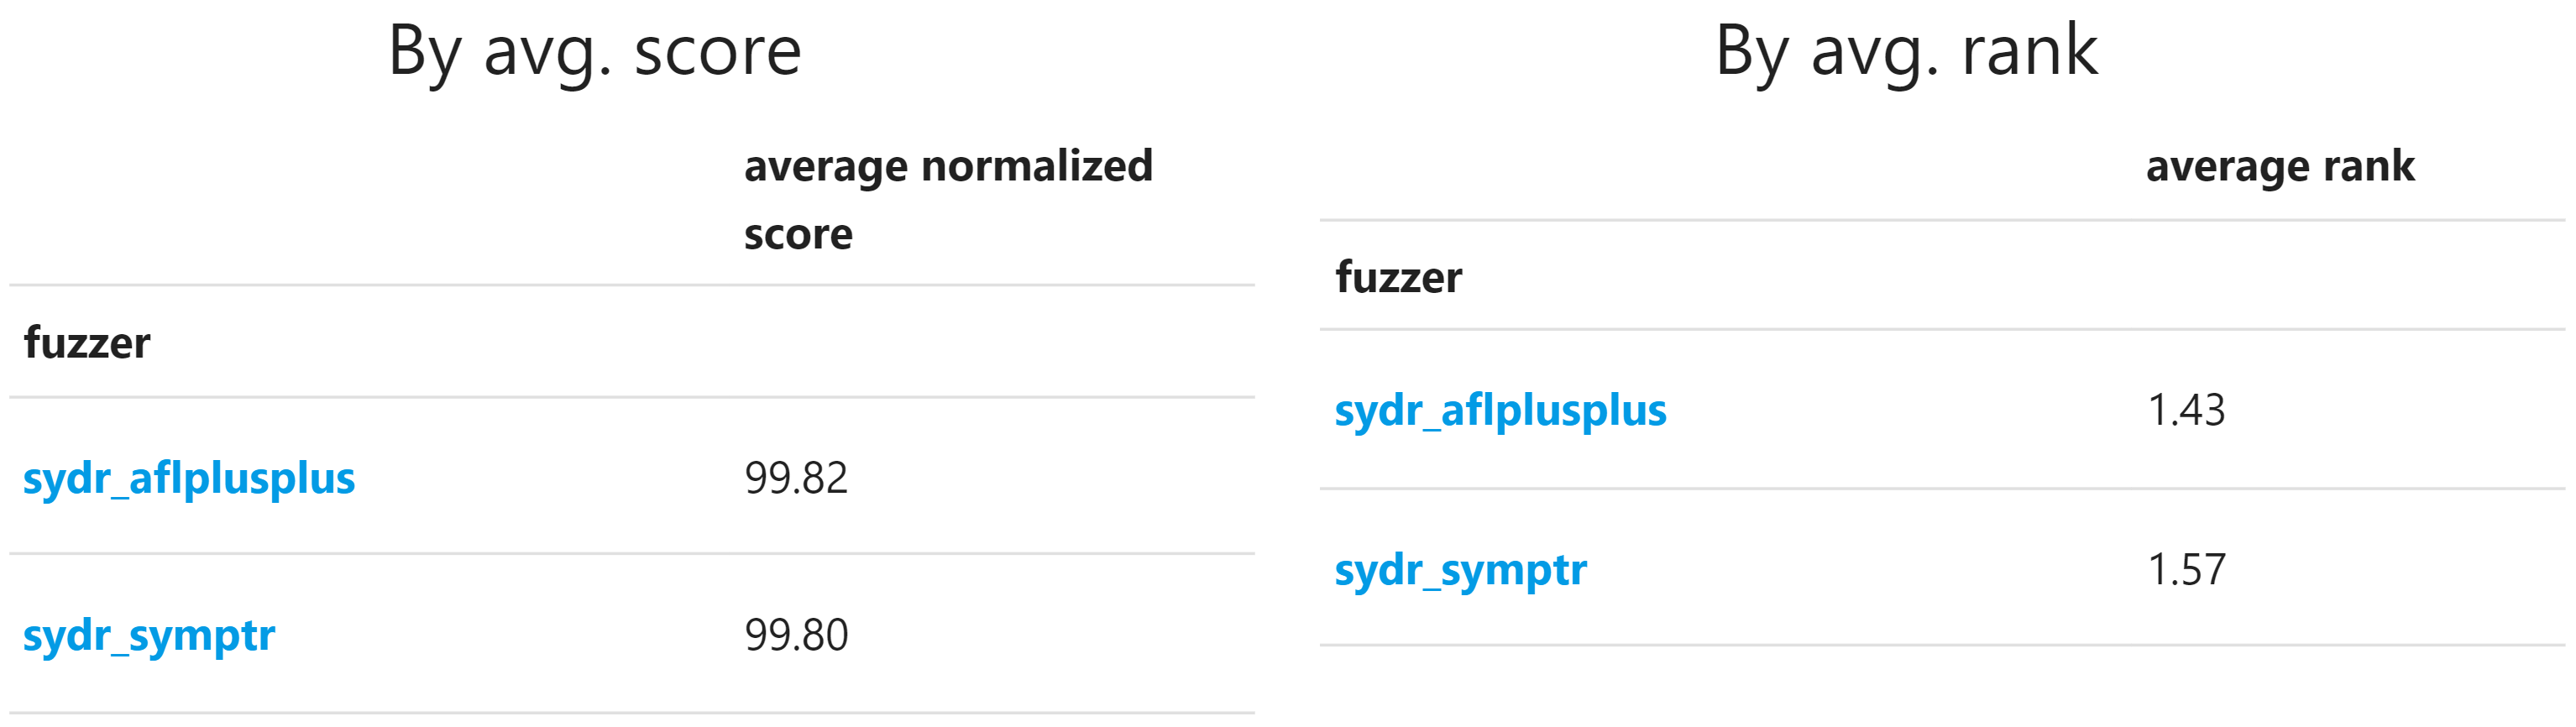
\includegraphics[width=0.9\textwidth]{assets/fuzzbench/symptr-15-1/avg-score-avg-rank.png}
    \caption{Average score and average rank ($N=15$)}
    \label{fig:fuzzbench-symptr-15-1-score-rank}
\end{figure}

As we can see from the results, the average score for the Sydr with enabled memory modeling ($N=15$) is 99.8 which is almost the same as the average score for the Sydr with disabled memory modeling (99.82), so with $N=15$ the scheduling strategy does not provide any significant improvements. The same is proved by the median relative code coverage.

\subsubsection{symptr-25}

The next configuration used $ N = 25 $. The results are shown in Figures \ref{fig:fuzzbench-symptr-25-1-coverage} and \ref{fig:fuzzbench-symptr-25-1-score-rank}. Coverage growth graphs can be found in Appendix \ref{fig:fuzzbench:symptr-25-1}.

\begin{figure}[h]
    \centering
    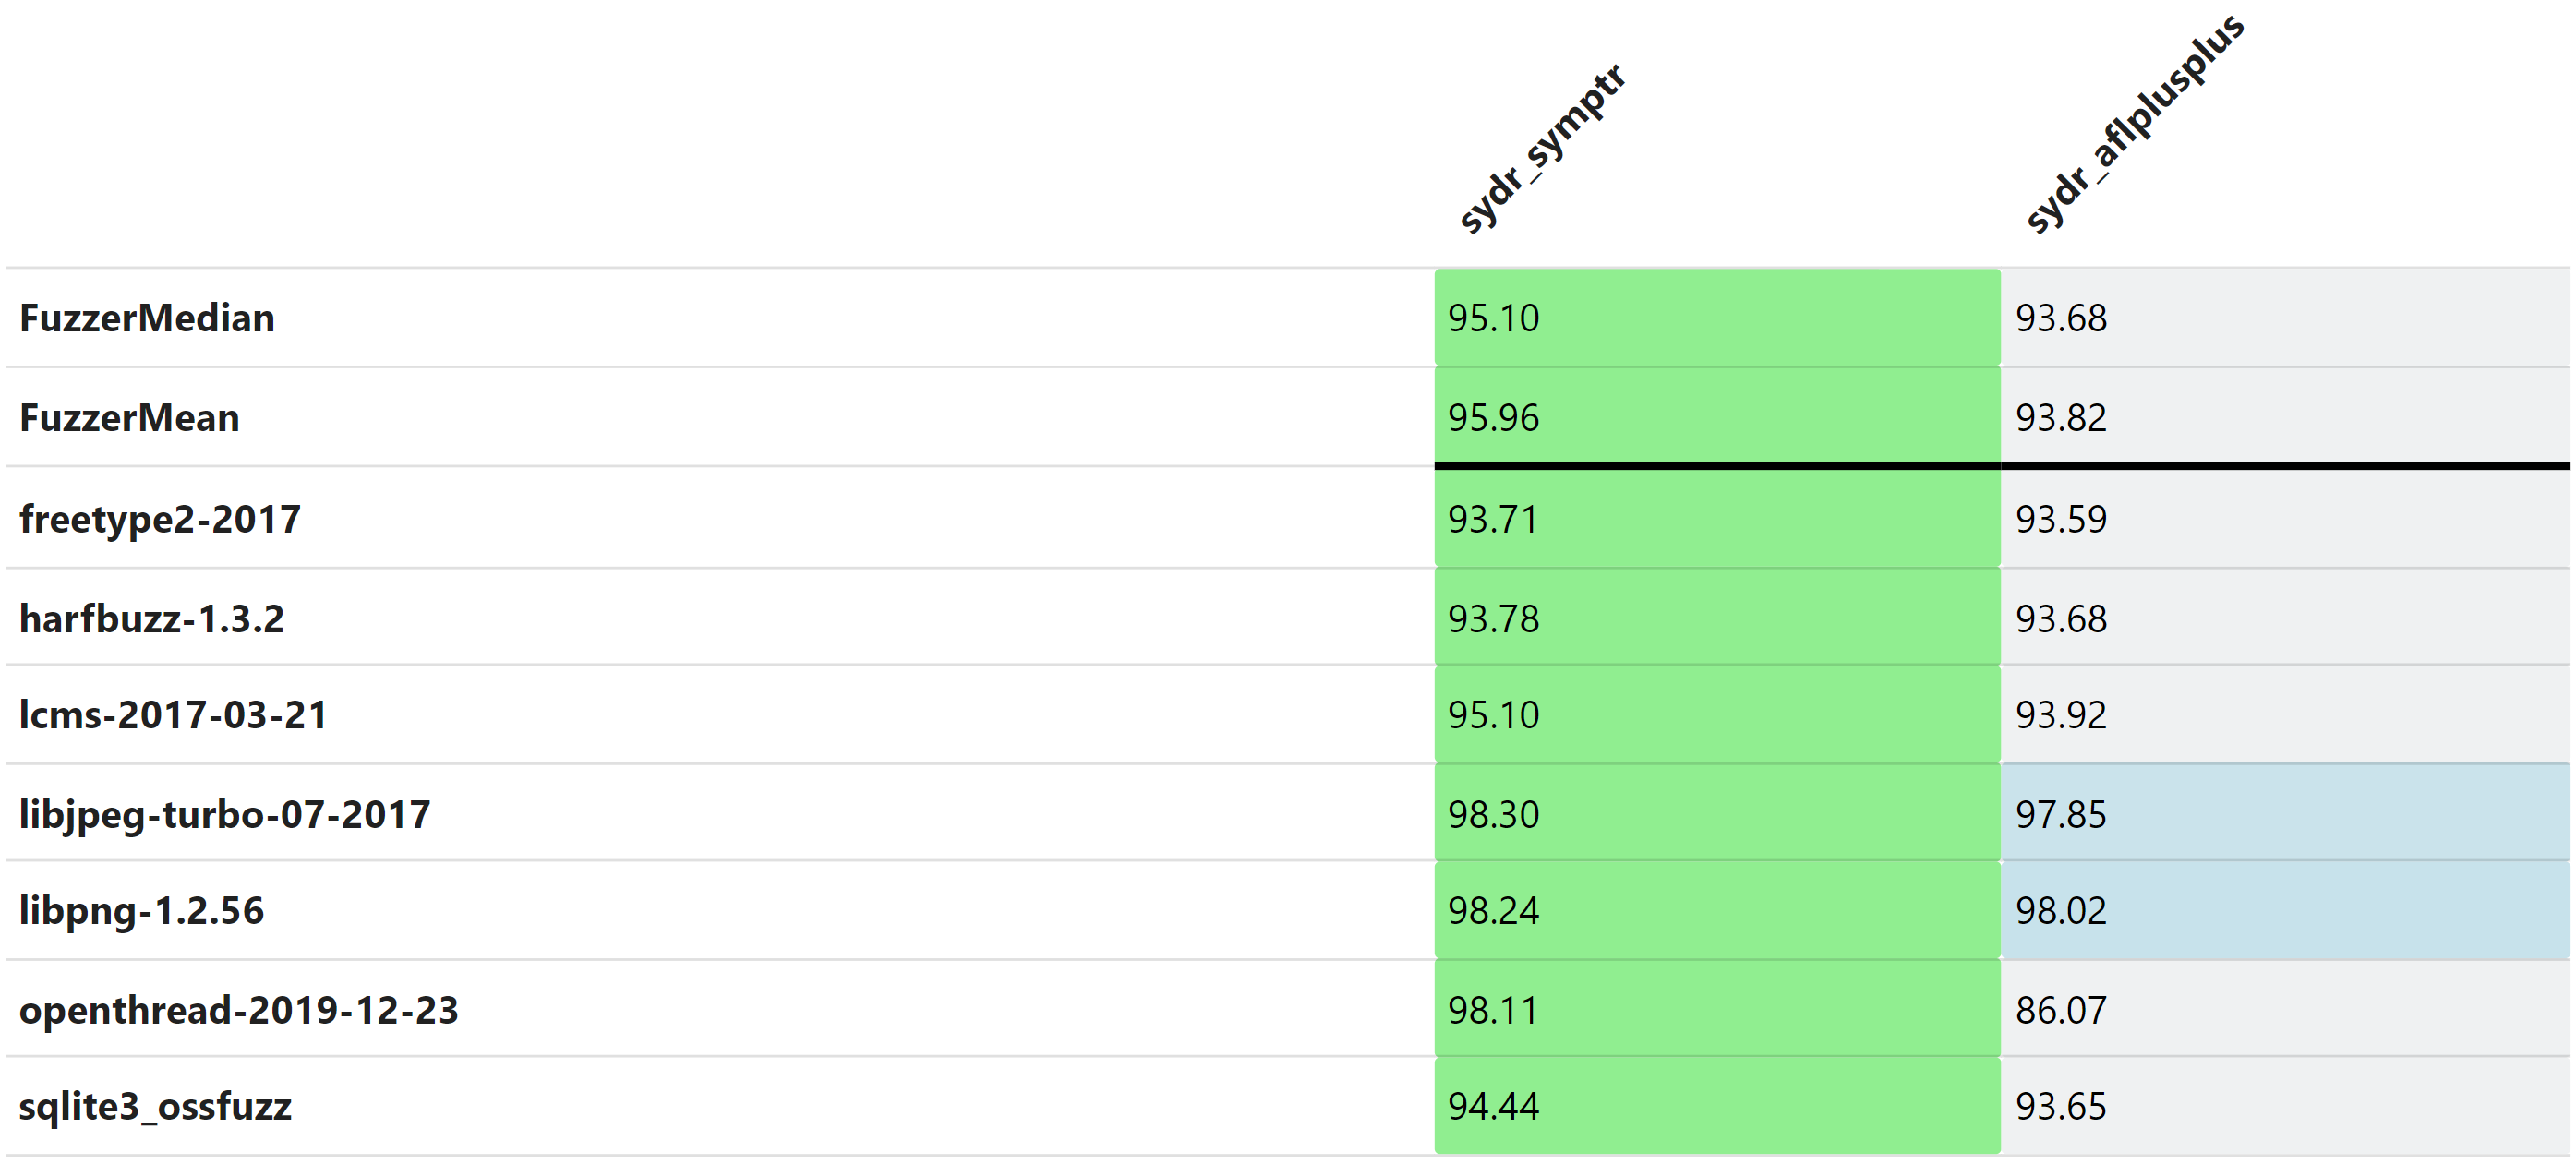
\includegraphics[width=0.9\textwidth]{assets/fuzzbench/symptr-25-1/median-relative-code-coverage-on-each-benchmark.png}
    \caption{Median relative code coverage on each benchmark ($N=25$)}
    \label{fig:fuzzbench-symptr-25-1-coverage}
\end{figure}

\begin{figure}[h]
    \centering
    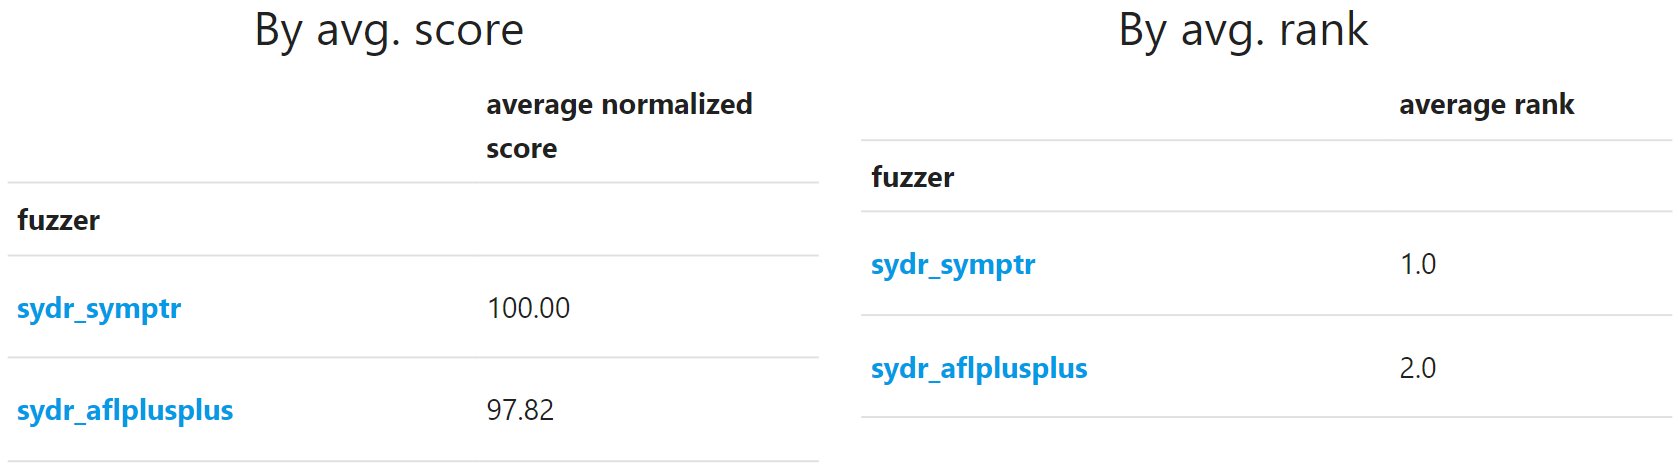
\includegraphics[width=0.9\textwidth]{assets/fuzzbench/symptr-25-1/avg-score-avg-rank.png}
    \caption{Average score and average rank ($N=25$)}
    \label{fig:fuzzbench-symptr-25-1-score-rank}
\end{figure}

This experiment showed much more promising results. The Sydr with enabled memory modeling ($N=25$) achieved an average score of 100.0, which is higher than the average score of 97.82 obtained by the Sydr with disabled memory modeling. The median relative code coverage table also shows that the scheduling strategy with $N=25$ yields better results, winning on all benchmarks.

\subsubsection{symptr-35-vs-25}

Finally, to decide whether we should use $ N = 25 $ or something higher (e.g. $ N = 35 $), we have conducted the third experiment. This time both instances used a scheduling strategy, but one of them used $ N = 25 $ and the other one used $ N = 35 $.

The results for the third configuration are shown in Figures \ref{fig:fuzzbench-symptr-25-vs-35-2-coverage} and \ref{fig:fuzzbench-symptr-25-vs-35-2-score-rank}. Coverage growth graphs for this experiment also can be found in Appendix \ref{fig:fuzzbench:symptr-25-vs-35-2}.

\begin{figure}[h]
    \centering
    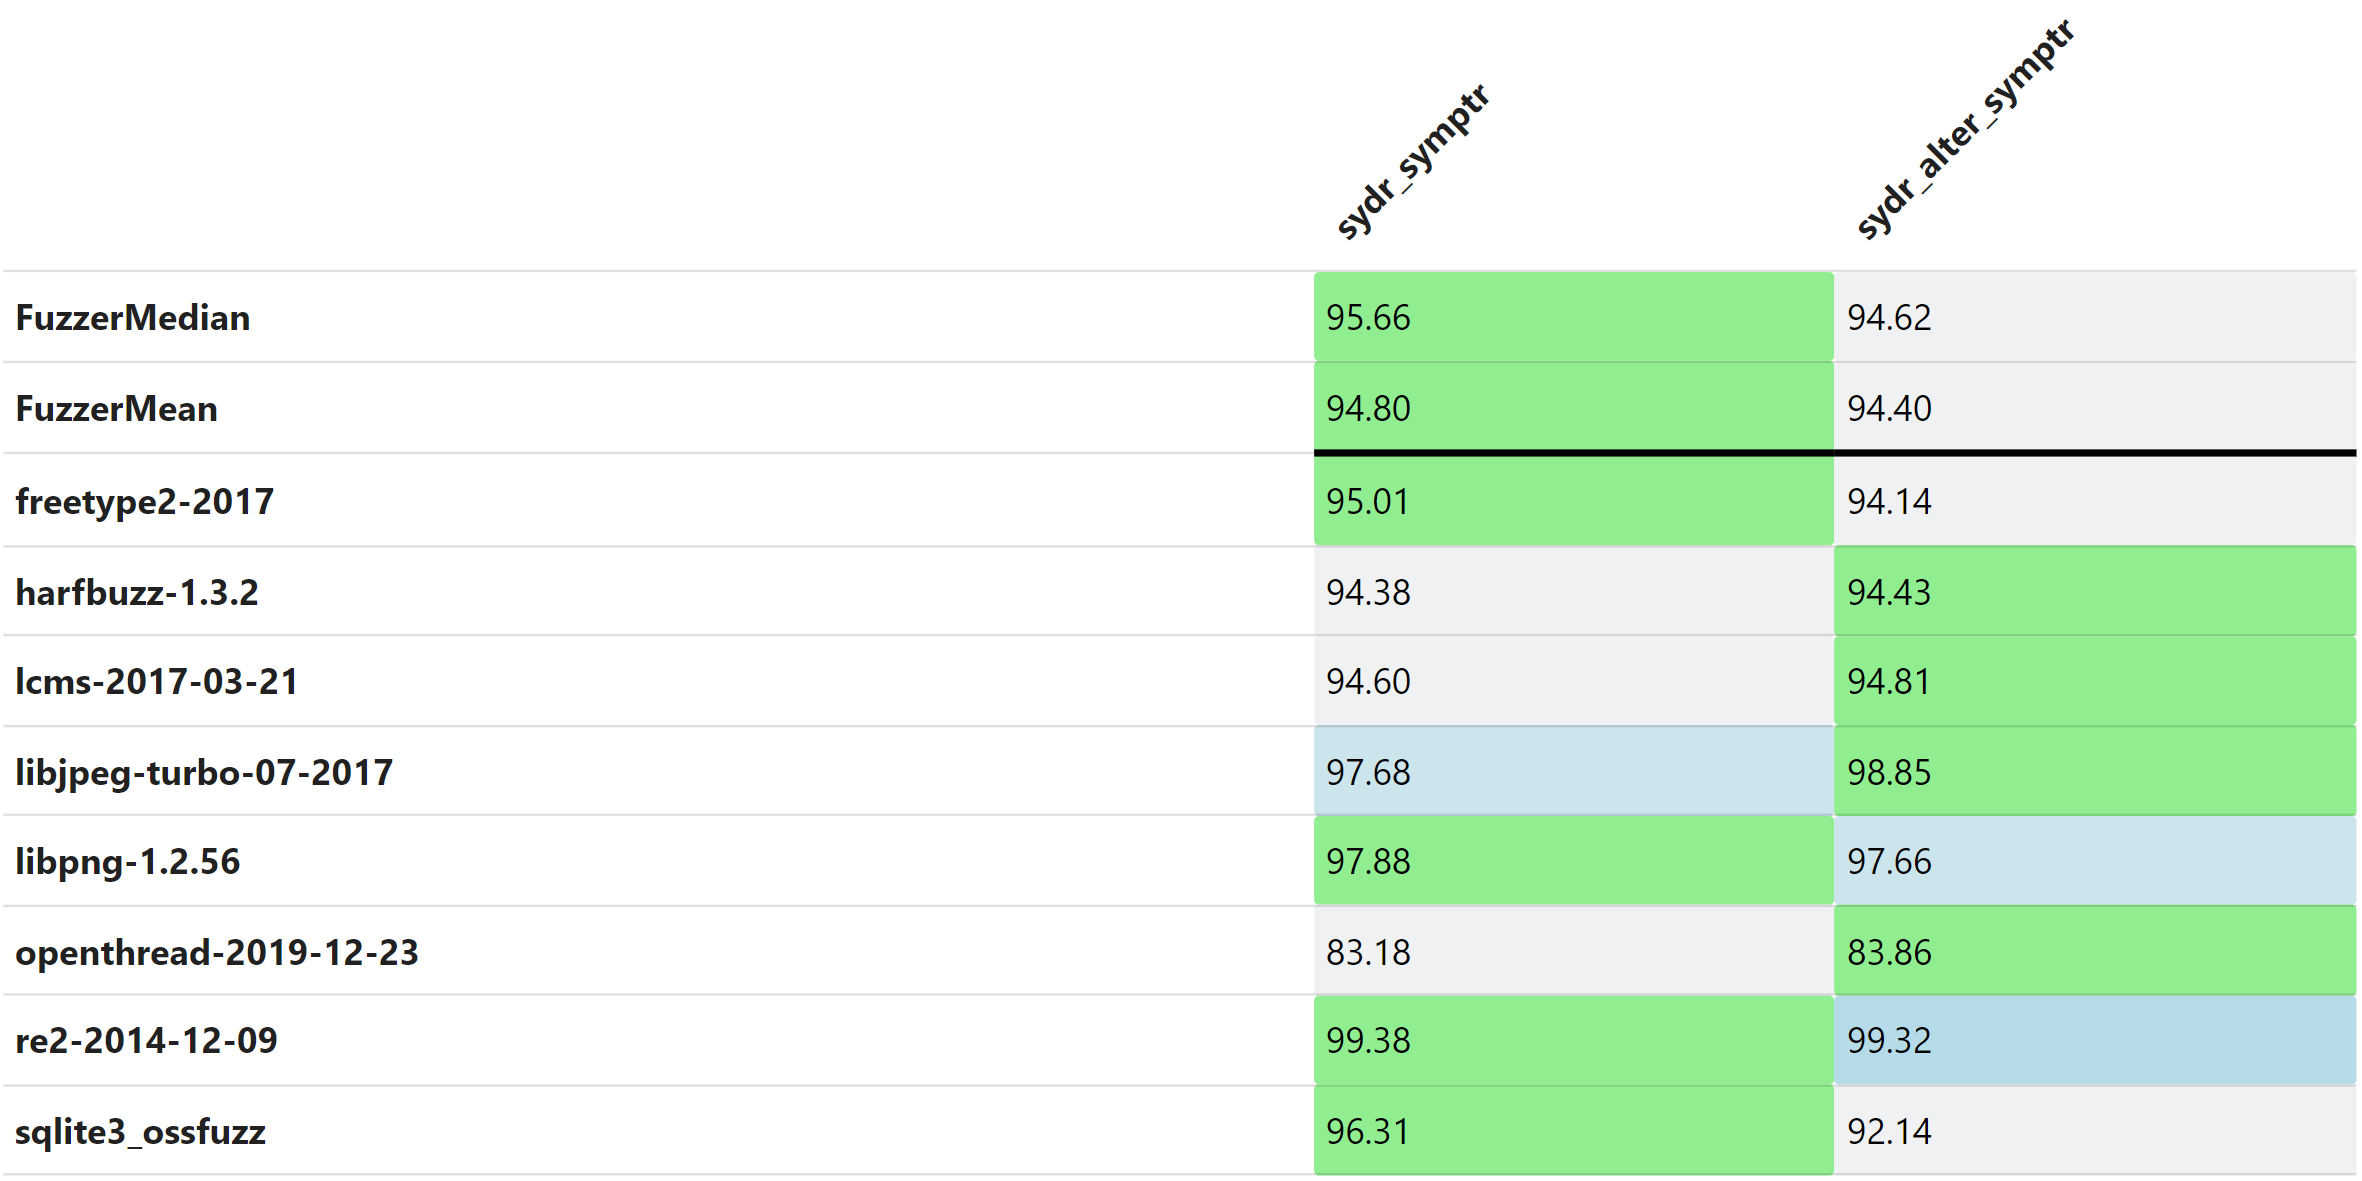
\includegraphics[width=0.9\textwidth]{assets/fuzzbench/symptr-25-vs-35-2/median-relative-code-coverage-on-each-benchmark.png}
    \caption{Median relative code coverage on each benchmark (N=25 vs N=35)}
    \label{fig:fuzzbench-symptr-25-vs-35-2-coverage}
\end{figure}

\begin{figure}[h]
    \centering
    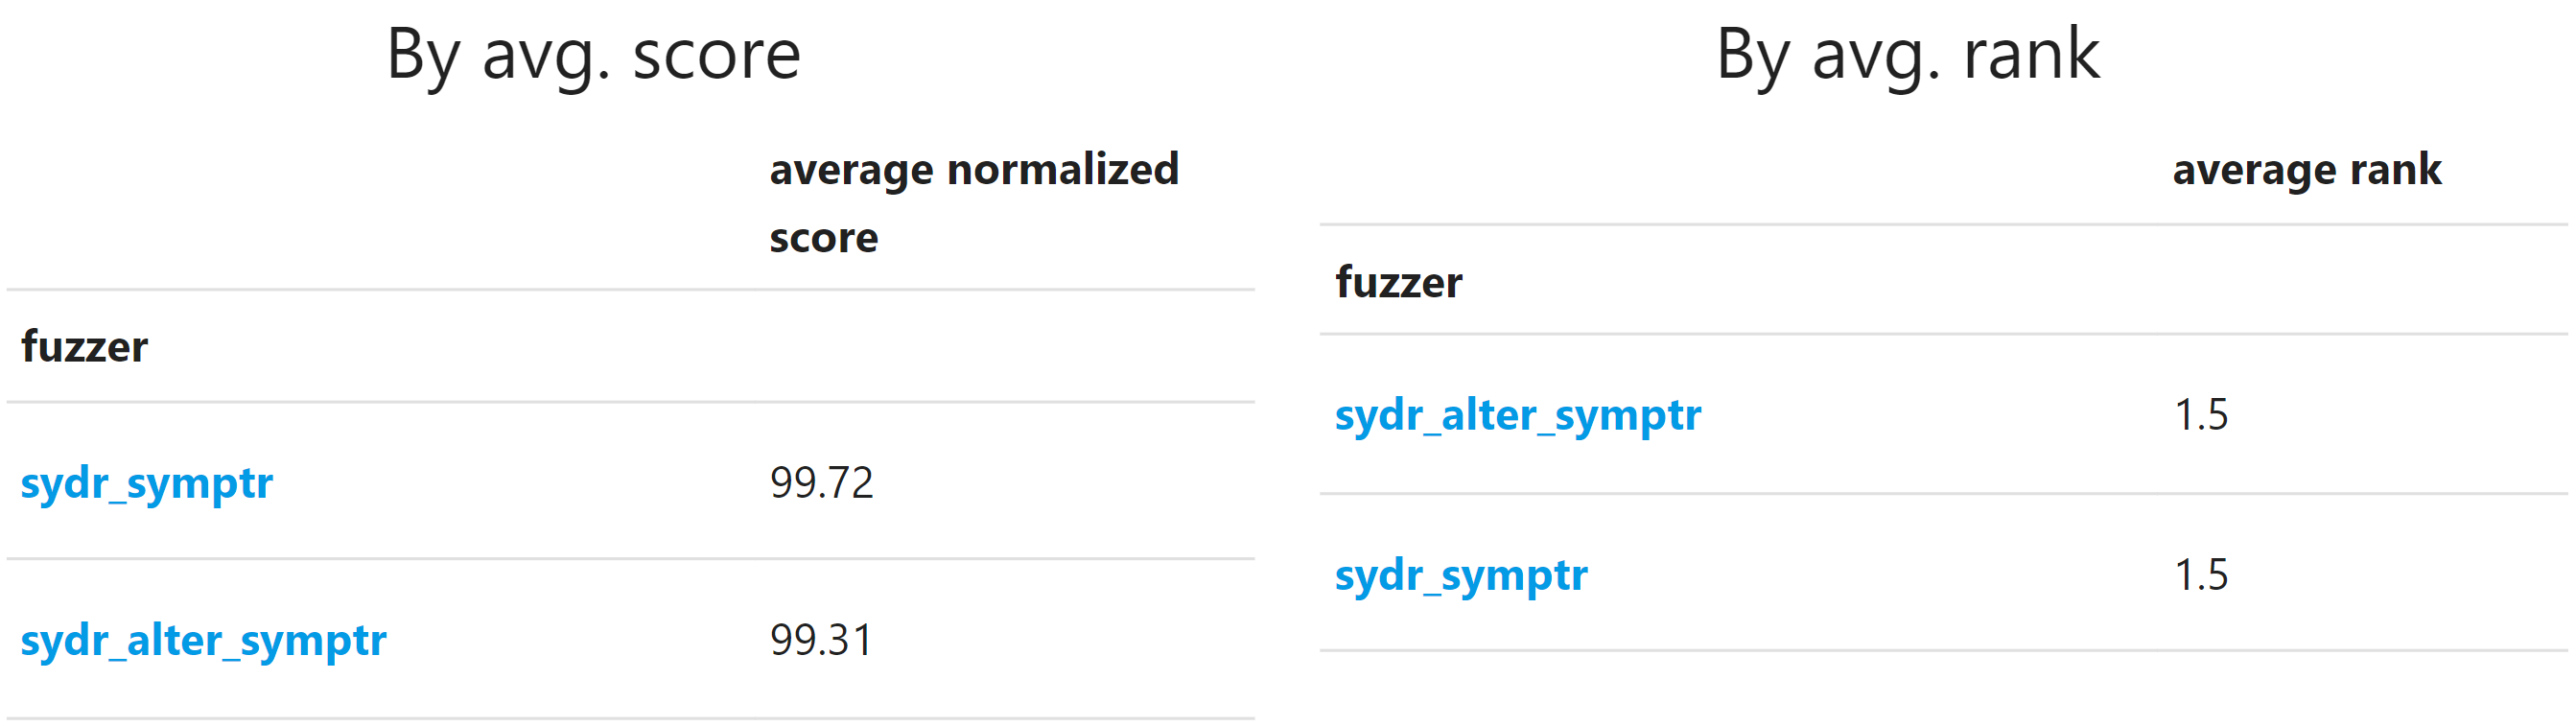
\includegraphics[width=0.9\textwidth]{assets/fuzzbench/symptr-25-vs-35-2/avg-score-avg-rank.png}
    \caption{Average score and average rank (N=25 vs N=35)}
    \label{fig:fuzzbench-symptr-25-vs-35-2-score-rank}
\end{figure}

As can be seen from the normalized average score, the Sydr with enabled memory modeling and $N=25$ is a little better than the one with $N=35$.

From this, we can conclude that the value of $N=25$ is indeed the most optimal for the scheduling strategy.

\subsection{Security Predicates Enchantment: Log Annotation} \label{results:security-invariants-enchantment-log-annotation}

The last, but not the least contribution of this thesis is the enchantment of security predicates with an improved log annotation mechanism.

To test the performance of the improved annotation mechanism, we have conducted several experiments, on various types of traces obtained from various programs. These experiments consist of two parts:

\begin{enumerate}
    \item Comparison of the previous method with the new one on branch traces obtained with the help of Sydr.
    \item Comparison of the previous method with the new one on instruction traces also obtained with the help of Sydr.
\end{enumerate}

The results of the first experiment are shown in Table \ref{table:annotate-branch-traces-10}. In this experiment, both methods were applied to annotate 10 branch traces obtained from the Sydr. The table shows the average time spent on annotation in milliseconds, as well as the standard deviation. The last column shows the performance difference between the two methods, which is calculated as follows:

$$ \frac{t_{old} - t_{new}}{t_{old}} \times 100 \% $$

where $t_{old}$ is the average time spent on annotation using the previous method and $t_{new}$ is the average time spent on annotation using the new method.

\definecolor{Gray}{gray}{0.9}
\newcolumntype{g}{>{\columncolor{Gray}}c}
\begin{table}[h]
    \centering
    \begin{tabular}{cgcgcg}
        \toprule
        \multirow{2}{*}{\bfseries Benchmark} & \multicolumn{2}{c}{\bfseries Default (ms)} & \multicolumn{2}{c}{\bfseries Rust (ms)} & \textbf{Performance diff}                            \\
                                             & Mean                                       & Std                                     & Mean                      & Std          &           \\
        cjson                                & 292.25                                     & $ \pm 66.1337 $                         & 1.08                      & $ \pm 0.06 $ & -99.63 \% \\
        libjpeg                              & 931.96                                     & $ \pm 55.3113 $                         & 1.75                      & $ \pm 0.19 $ & -99.81 \% \\
        libpng                               & 924.03                                     & $ \pm 567.277 $                         & 1.64                      & $ \pm 0.26 $ & -99.82 \% \\
        libxml2                              & 38308.54                                   & $ \pm 796.162 $                         & 12.27                     & $ \pm 0.33 $ & -99.97 \% \\
        minigzip                             & 14567.67                                   & $ \pm 121.165 $                         & 7.51                      & $ \pm 0.48 $ & -99.94 \% \\
        pcre2                                & 14562.59                                   & $ \pm 1419.99 $                         & 7.26                      & $ \pm 0.58 $ & -99.95 \% \\
        readelf                              & 19486.86                                   & $ \pm 1015.72 $                         & 7.02                      & $ \pm 0.36 $ & -99.96 \% \\
        rizin                                & 31061.09                                   & $ \pm 1800.72 $                         & 12.77                     & $ \pm 0.22 $ & -99.96 \% \\
        yices                                & 8936.02                                    & $ \pm 111.98 $                          & 3.98                      & $ \pm 0.3 $  & -99.96 \% \\
        yodl                                 & 16907.58                                   & $ \pm 377.37 $                          & 7.97                      & $ \pm 0.31 $ & -99.95 \% \\
        \bottomrule
    \end{tabular}
    \caption{Mean execution time to annotate 10 branch traces with the default and Rust annotator.}
    \label{table:annotate-branch-traces-10}
\end{table}

This experiment shows that the new method is significantly faster than the previous one. The average performance difference is close to 99.9\%.

The second experiment tested the performance of the new method on instruction trace. The results of this experiment are shown in Table \ref{table:annotate-instruction-trace-3}. The table shows the average time spent on annotation in seconds, as well as the standard deviation across 3 runs. The last column shows the performance difference between the two methods, which is calculated in the same way as in the previous experiment.

As on average instruction traces are much larger than branch traces, some benchmarks were not able to finish within a given time limit of 30 minutes. Therefore, some lines in the table are marked with a \textit{timeout}.

\definecolor{Gray}{gray}{0.9}
\newcolumntype{g}{>{\columncolor{Gray}}c}
\begin{table}[h]
    \centering
    \resizebox{\columnwidth}{!}{%
        \begin{tabular}{ccgcgcg}
            \toprule
            \multirow{2}{*}{\bfseries Benchmark} & \multirow{2}{*}{\bfseries Size (mb)} & \multicolumn{2}{c}{\bfseries Default (s)} & \multicolumn{2}{c}{\bfseries Rust (s)} & \textbf{Performance diff}                             \\
                                                 &                                      & Mean                                      & Std                                    & Mean                      & Std           &           \\
            cjson                                & 1.21                                 & 20.74                                     & $ \pm 0.05 $                           & 0.23                      & $ \pm 0.005 $ & -98.87 \% \\
            libjpeg                              & 6.69                                 & 176.9                                     & $ \pm 0.60 $                           & 2.32                      & $ \pm 0.027 $ & -98.69 \% \\
            libpng                               & 2.08                                 & 57.6                                      & $ \pm 0.36 $                           & 0.75                      & $ \pm 0.019 $ & -98.69 \% \\
            libxml2                              & 50.3                                 & timeout                                   & timeout                                & 21.27                     & $ \pm 1.016 $ & XXX \%    \\
            minigzip                             & 0.75                                 & timeout                                   & timeout                                & 166.59                    & $ \pm 1.863 $ & XXX \%    \\
            pcre2                                & 6.62                                 & 172.77                                    & $ \pm 0.69 $                           & 2.8                       & $ \pm 0.048 $ & -98.38 \% \\
            readelf                              & 9.19                                 & 454.11                                    & $ \pm 40.68 $                          & 3.94                      & $ \pm 0.144 $ & -99.13 \% \\
            rizin                                & 34.04                                & timeout                                   & timeout                                & 15.15                     & $ \pm 0.925 $ & XXX \%    \\
            yices                                & 10.48                                & 294                                       & $ \pm 1.1 $                            & 4.69                      & $ \pm 0.123 $ & -98.4 \%  \\
            yodl                                 & 22.53                                & timeout                                   & timeout                                & 10.3                      & $ \pm 1.014 $ & XXX \%    \\
            \bottomrule
        \end{tabular}
    }
    \caption{Mean execution time (over 3 runs) to annotate instruction trace with the default and Rust annotator.}
    \label{table:annotate-instruction-trace-3}
\end{table}

For this type of trace, the performance is still incomparably higher than the previous method. The average performance difference is close to 98.7\%.

Overall, the new method is significantly faster than the previous one on all benchmarks. The improvements in this module allow us to substantially improve the performance of the whole verification process.

This concludes the discussion about the results achieved in this thesis.
